\documentclass{beamer}
\usepackage[utf8]{inputenc}

\title{Prompt Engineering - Mini Projekt}
\author{Jan Albrecht}
\date{January 2021}

\usepackage[utf8]{inputenc}
\usepackage{ulem}
\usepackage{utopia} %font utopia imported
\usepackage{amssymb,nccmath,float}
\usepackage{amsmath,mathtools}
\usepackage[style=numeric,maxalphanames=1,backend=biber]{biblatex}
\usepackage{wrapfig}
\usepackage[font=footnotesize]{caption}
\DeclarePairedDelimiter\ceil{\lceil}{\rceil}
\DeclarePairedDelimiter\floor{\lfloor}{\rfloor}

\usetheme{Madrid}
\definecolor{UBCblue}{rgb}{0.04706, 0.13725, 0.26667}
\definecolor{forestgreen}{RGB}{34,139,34}
\usecolortheme[named=UBCblue]{structure}


%------------------------------------------------------------
\renewcommand*{\labelalphaothers}{}

\DeclareLabelalphaTemplate{
	\labelelement{
		\field[final]{shorthand}
		\field{labelname}
		\field{label}
	}
	\labelelement{
		\literal{\addhighpenspace}
	}
	\labelelement{
		\field{year}
	}
}


%------------------------------------------------------------
%This block of code defines the information to appear in the
%Title page
\title[Prompt Engineering Project] %optional
{Taxonomy Exploration - Map of Mathematics}
\subtitle{Finding Superordinate Topics in Mathematics}



\author[J. Albrecht] % (optional)
{Jan Albrecht}

\institute[Student - University Leipzig] % (optional)
{University Leipzig}

\date[12.06.2022] % (optional)


\logo{\includegraphics[height=1.5cm]{images/512px-Universität_Leipzig_logo.svg.png}}

%------------------------------------------------------------
\begin{document}
	%The next statement creates the title page.
	\frame{\titlepage}
	%---------------------------------------------------------
	\section{Example Prompt}
	\begin{frame}{Example Prompt \& Output in \textit{text-davinci-002}}
		\begin{wrapfigure}{l}{0.4\textwidth}
			\fbox{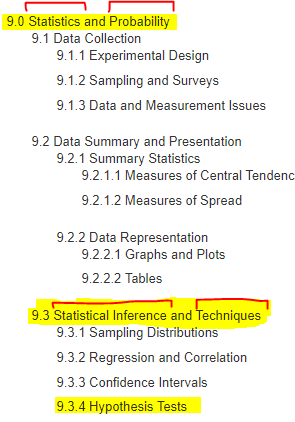
\includegraphics[width=0.78\linewidth]{./images/taxonomy.png}}
			\captionsetup[wrapfigure]{font=small}
			\caption{This taxonomy is based on the Math NSDL Taxonomy Committee Report, April 2, 2002}
			\label{fig:tax}
		\end{wrapfigure}

		\textit{Mathematical topics are strongly connected, for example the hypernym of \textbf{Hypothesis Tests} is called} \color{forestgreen} \textbf{Statistical Inference}\\[30pt] \color{black}
	
		X = ''Hypothesis Tests''\\[6pt]
		y $\in Y$ = $\{$''Statistical Interference'', ''Techniques'', ''Statistics'', ''Probability''$\}$\\[6pt]
		$s(y,\hat{y})$ = $1 - \frac{min(dist_{LV}(y, \hat{y}))}{max(len(y),len(\hat{y}))}$ for $y \in Y$\\[48pt]
	\end{frame}
	%---------------------------------------------------------
\section{Investigation}
\begin{frame}{Investigation}
	\begin{figure}[hbtp]
		\centering
		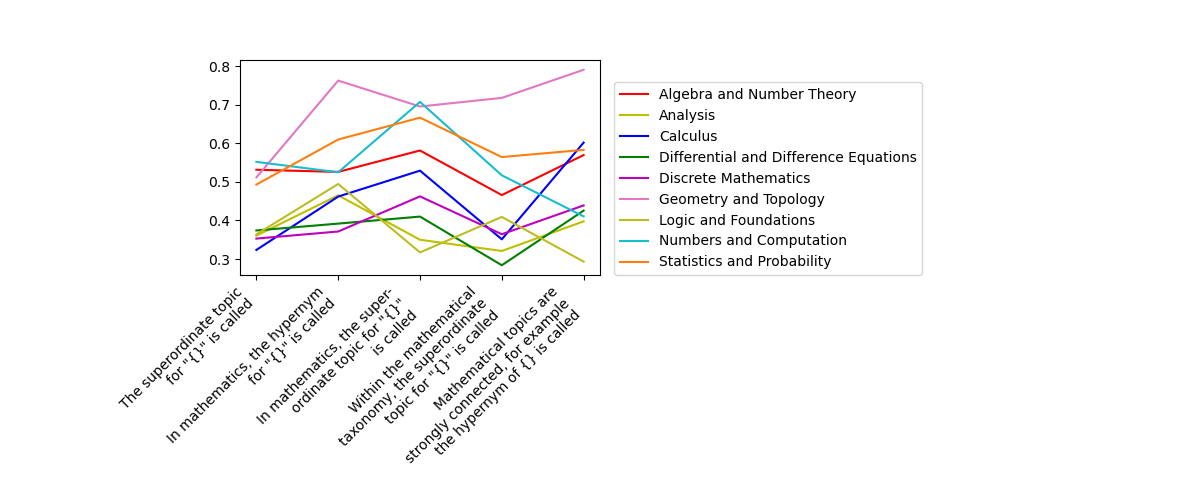
\includegraphics[width=1.3\linewidth]{./images/Model.png}
		\caption{Model Performance}
		\label{fig:model}
	\end{figure}
\end{frame}
\end{document}
